\chapter{Stereochemie verdiept}\label{ch:b1:stereochemistry-in-depth}

Kneus een paar karwijzaadjes, en daarna een blad groene munt: twee heel
verschillende geuren. De belangrijkste geurstof van elk is carvon,
\ce{C10H14O}, dezelfde atomen in dezelfde volgorde verbonden --- maar de
twee carvonen zijn elkaars spiegelbeeld, zoals een linkerhand dat is van
een rechterhand, en de receptoren van de neus, zelf opgebouwd uit
spiegelasymmetrische moleculen, onderscheiden ze. Geneesmiddelen,
smaakstoffen en de moleculen van het leven zijn allemaal driedimensionaal
gebouwd, en een structuurformule die de derde dimensie negeert, mist de
helft van het verhaal. Dit hoofdstuk geeft de werktuigen om moleculen in
de ruimte te tekenen, om elke schikking ondubbelzinnig te benoemen, om de
rotaties te volgen die moleculen voortdurend uitvoeren, en om de enige
fysische eigenschap te meten die spiegelbeelden van elkaar onderscheidt.

\begin{recall}
Het schoolboek (jaar 12) voerde \omterm{def:b1:stereochemistry-in-depth:stereocentre}{chirale} moleculen in, het asymmetrische
koolstofatoom, \omterm{def:b1:stereochemistry-in-depth:enantiomers}{enantiomeren}, $Z$/$E$-isomeren en de \omterm{def:b1:stereochemistry-in-depth:isomers}{conformaties} van
ethaan. De tetraëdrische schikking van vier bindingen rond koolstof en de
beschrijving van enkele en dubbele bindingen met
$\sigma$/$\pi$ komen uit \cref{ch:b1:lewis-resonance-vsepr}.
\end{recall}

\begin{omfigure}
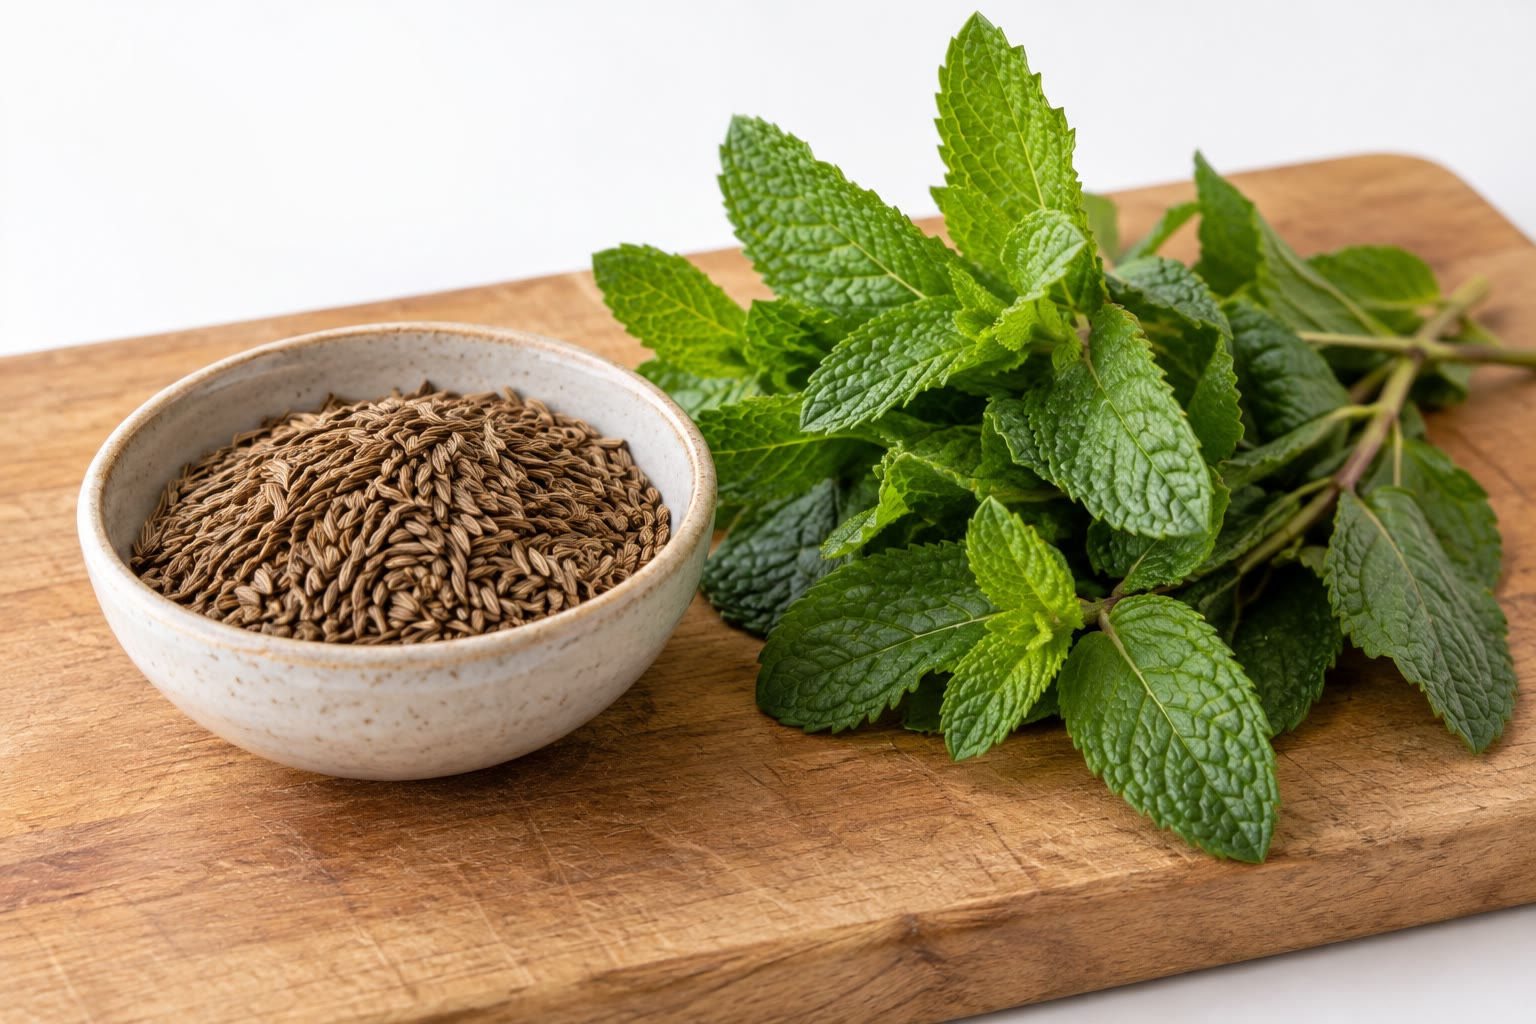
\includegraphics[width=0.55\linewidth]{images/book2/ai/b1-16-caraway-mint.jpg}

{\small Karwijzaad en blaadjes groene munt. Karwij dankt zijn geur
vooral aan \cip{S}-carvon, groene munt aan het spiegelbeeld daarvan,
\cip{R}-carvon.}
\end{omfigure}

\section{Isomeren en voorstellingen}

\begin{definition}[Constitutie, configuratie, conformatie]\label{def:b1:stereochemistry-in-depth:isomers}
Twee verbindingen met dezelfde formule waarvan de atomen in een andere
volgorde verbonden zijn, zijn
\emph{constitutie-isomeren}\index{constitutie-isomeren}. Verbindingen met
dezelfde constitutie waarvan de atomen alleen verschillen in hun
schikking in de ruimte, zijn
\emph{stereo-isomeren}\index{stereo-isomeren}. De schikking die alleen
veranderd kan worden door bindingen te verbreken, is de
\emph{configuratie}\index{configuratie} van een stereo-isomeer; een
schikking die verkregen wordt door rotatie om enkele bindingen, zonder er
een te verbreken, is een \emph{conformatie}\index{conformatie}.
\end{definition}

Bij kamertemperatuur vinden rotaties om enkele bindingen miljarden keren
per seconde plaats: \omterm{def:b1:stereochemistry-in-depth:isomers}{conformaties} gaan in elkaar over en kunnen niet
geïsoleerd worden, terwijl \omterm{def:b1:stereochemistry-in-depth:isomers}{configuraties} stabiel zijn en verschillende
verbindingen geven.

\begin{definition}[Voorstellingen]\label{def:b1:stereochemistry-in-depth:representations}
In de \emph{weergave volgens Cram}\index{weergave volgens Cram} worden
twee bindingen in het vlak van het papier getekend, wijst een volle wig
naar de lezer toe en een gearceerde wig van de lezer af. Een
\emph{newmanprojectie}\index{newmanprojectie} bekijkt een molecuul langs
één C--C-binding: het voorste koolstofatoom is een punt waar zijn drie
andere bindingen samenkomen, het achterste een cirkel uit de rand
waarvan zijn bindingen vertrekken. In een
\emph{fischerprojectie}\index{fischerprojectie} staat de koolstofketen
verticaal, wijzen horizontale bindingen naar de lezer toe en verticale
bindingen van de lezer af; elk kruispunt is een stereogeen
koolstofatoom.
\end{definition}

\begin{omfigure}
\begin{tikzpicture}[font=\small]
  % staggered and eclipsed ethane, Newman
  \pic (s) at (0,0) {omnewman={90}{30}};
  \foreach \k in {1,2,3} { \node at (s-f\k) {H}; \node at (s-b\k) {H}; }
  \node at (0,-1.9) {gestaffeld};
  \pic (e) at (3.6,0) {omnewman={90}{108}};
  \foreach \k in {1,2,3} { \node at (e-f\k) {H}; }
  \foreach \k in {1,2,3} { \node[font=\scriptsize, black!60] at ($(e-b\k)!-0.12!(e-c)$) {H}; }
  \node at (3.6,-1.9) {eclips};
  % Fischer projection of (R)-lactic acid
  \begin{scope}[xshift=7.6cm]
    \draw[thick] (-0.9,0) -- (0.9,0) (0,-0.9) -- (0,0.9);
    \node[above] at (0,0.9) {\ce{COOH}};
    \node[below] at (0,-0.9) {\ce{CH3}};
    \node[left] at (-0.9,0) {H};
    \node[right] at (0.9,0) {OH};
    \node at (0,-1.9) {Fischer};
  \end{scope}
  % Cram of the same
  \begin{scope}[xshift=11.0cm]
    \node at (0,0) {\chemfig{C(-[2]COOH)(-[:210]H_3C)(<:[:-12]OH)(<[:-55]H)}};
    \node at (0,-1.9) {Cram};
  \end{scope}
\end{tikzpicture}

{\small Links: \omterm{def:b1:stereochemistry-in-depth:representations}{newmanprojecties} van ethaan langs zijn C--C-binding,
gestaffeld (achterste bindingen tussen de voorste) en eclips (achterste
bindingen verborgen achter de voorste, iets verschoven getekend). Rechts:
hetzelfde molecuul, \cip{R}-melkzuur, als \omterm{def:b1:stereochemistry-in-depth:representations}{fischerprojectie} en in de
\omterm{def:b1:stereochemistry-in-depth:representations}{weergave volgens Cram} (de verticale bindingen van het fischerkruis
wijzen van de lezer af, de horizontale naar de lezer toe).}
\end{omfigure}

\begin{method}[Van Cram naar Newman]\label{met:b1:stereochemistry-in-depth:newman-from-cram}
\begin{enumerate}
  \item Kies de binding waarlangs je kijkt en het uiteinde dat het dichtst
        bij het oog ligt.
  \item Teken de drie bindingen van het voorste koolstofatoom vanuit het
        middelpunt, met behoud van hun volgorde (met of tegen de wijzers
        van de klok in) zoals het oog ze ziet.
  \item Teken de bindingen van het achterste koolstofatoom vanaf de
        cirkel, met hun volgorde zoals ze vanaf dezelfde kant gezien
        worden.
  \item Controleer: het achterste koolstofatoom $60^\circ$ draaien gaat van
        gestaffeld naar eclips; $120^\circ$ van de ene \omterm{def:b1:stereochemistry-in-depth:conformations}{gestaffelde
        conformatie} naar de volgende.
\end{enumerate}
\end{method}

\section{Configuratie: de CIP-regels}

\begin{definition}[CIP-regels, descriptoren]\label{def:b1:stereochemistry-in-depth:cip}
De \emph{CIP-regels}\index{CIP-regels} (Cahn--Ingold--Prelog) rangschikken
de vier substituenten van een \omterm{def:b1:stereochemistry-in-depth:stereocentre}{stereogeen centrum}: eerst het hogere
atoomnummer; bij gelijkheid vergelijk je de verzamelingen atomen die
daarna gebonden zijn, en zo verder naar buiten; een dubbele binding telt
als twee enkele bindingen naar gedupliceerde atomen. Met de laagst
gerangschikte substituent van het oog af gericht definieert de volgorde
$1 \to 2 \to 3$ met de wijzers van de klok mee de descriptor \cip{R}, en
tegen de wijzers van de klok in \cip{S}. Voor een dubbele binding met
twee substituenten op elk koolstofatoom betekent \cip{Z} dat de twee
hoogst gerangschikte aan dezelfde kant staan, en \cip{E} aan
tegengestelde kanten.
\end{definition}

\begin{method}[\texorpdfstring{\cip{R}}{(R)} of \texorpdfstring{\cip{S}}{(S)} toekennen]\label{met:b1:stereochemistry-in-depth:cip}
\begin{enumerate}
  \item Rangschik de vier substituenten met de \omterm{def:b1:stereochemistry-in-depth:cip}{CIP-regels}.
  \item Wijst de laagst gerangschikte van je af (gearceerde wig, of een
        verticale binding van een \omterm{def:b1:stereochemistry-in-depth:representations}{fischerprojectie}), lees dan de draairichting
        van $1 \to 2 \to 3$ rechtstreeks af.
  \item Wijst ze naar je toe (volle wig, horizontale fischerbinding),
        lees dan de draairichting af en keer de descriptor om.
  \item Twee willekeurige substituenten verwisselen keert de descriptor
        om: een snelle controle.
\end{enumerate}
In melkzuur is $\ce{OH} > \ce{COOH} > \ce{CH3} > \ce{H}$ (O; daarna wint
C(O,O,O) van C(H,H,H)). In de \omterm{def:b1:stereochemistry-in-depth:representations}{fischerprojectie} hierboven staat H
horizontaal (naar ons toe) en draait $\ce{OH} \to \ce{COOH} \to \ce{CH3}$
tegen de wijzers van de klok in: omgekeerd is het centrum \cip{R}.
\end{method}

\section{Chiraliteit en de gevolgen ervan}

\begin{definition}[Stereogeen centrum, chiraliteit]\label{def:b1:stereochemistry-in-depth:stereocentre}
Een voorwerp is \emph{chiraal}\index{chiraal} als het niet met zijn
spiegelbeeld tot dekking gebracht kan worden, en anders
\emph{achiraal}\index{achiraal}; de eigenschap heet
\emph{chiraliteit}\index{chiraliteit}. Een \emph{stereogeen
centrum}\index{stereogeen centrum} is een atoom waarbij het verwisselen
van twee substituenten een \omterm{def:b1:stereochemistry-in-depth:isomers}{stereo-isomeer} geeft; een tetraëdrisch
koolstofatoom met vier verschillende substituenten is er een.
\end{definition}

Een molecuul met een spiegelvlak of een symmetriecentrum is \omterm{def:b1:stereochemistry-in-depth:stereocentre}{achiraal}; een
molecuul zonder een van beide is in de praktijk \omterm{def:b1:stereochemistry-in-depth:stereocentre}{chiraal}. Het exacte
criterium, uitgedrukt met symmetrieoperaties, wordt gegeven in het deel
van jaar~3.

\begin{definition}[Enantiomeren, diastereomeren, mesoverbinding, racemisch mengsel]\label{def:b1:stereochemistry-in-depth:enantiomers}
Twee \omterm{def:b1:stereochemistry-in-depth:isomers}{stereo-isomeren} die elkaars spiegelbeeld zijn, zijn
\emph{enantiomeren}\index{enantiomeren}; \omterm{def:b1:stereochemistry-in-depth:isomers}{stereo-isomeren} die dat niet
zijn, zijn \emph{diastereomeren}\index{diastereomeren}. Een
\emph{mesoverbinding}\index{mesoverbinding} heeft \omterm{def:b1:stereochemistry-in-depth:stereocentre}{stereogene centra} maar
is \omterm{def:b1:stereochemistry-in-depth:stereocentre}{achiraal}. Een equimolair mengsel van twee enantiomeren is een
\emph{racemisch mengsel}\index{racemisch mengsel}.
\end{definition}

\begin{proposition}[Aantal stereo-isomeren]\label{prop:b1:stereochemistry-in-depth:max-stereoisomers}
Een molecuul met $n$ \omterm{def:b1:stereochemistry-in-depth:stereocentre}{stereogene centra} (en geen andere stereogene
eenheid) heeft ten hoogste $2^n$ \omterm{def:b1:stereochemistry-in-depth:isomers}{stereo-isomeren}, in ten hoogste
$2^{n-1}$ paren \omterm{def:b1:stereochemistry-in-depth:enantiomers}{enantiomeren}; mesovormen maken het aantal kleiner.
\end{proposition}

\begin{proof}
Elk centrum is onafhankelijk \cip{R} of \cip{S}: $2^n$ combinaties. Het
spiegelbeeld verandert elke descriptor, zodat de combinaties paarsgewijs
\omterm{def:b1:stereochemistry-in-depth:enantiomers}{enantiomeren} vormen, $2^{n-1}$ paren. Is een combinatie na een rotatie
van het molecuul haar eigen spiegelbeeld (een mesovorm), dan valt haar
paar samen tot één verbinding.
\end{proof}

Wijnsteenzuur, \ce{HOOC-CH(OH)-CH(OH)-COOH}, heeft twee gelijkwaardige
centra: \cip{R,R} en \cip{S,S} zijn \omterm{def:b1:stereochemistry-in-depth:enantiomers}{enantiomeren}, terwijl \cip{R,S} een
spiegelvlak tussen de twee koolstofatomen heeft en meso is: drie
\omterm{def:b1:stereochemistry-in-depth:isomers}{stereo-isomeren}, geen vier.

\begin{proposition}[Eigenschappen van enantiomeren]\label{prop:b1:stereochemistry-in-depth:enantiomer-properties}
Twee \omterm{def:b1:stereochemistry-in-depth:enantiomers}{enantiomeren} hebben dezelfde smelt- en kookpunten, dezelfde
\omterm{def:b1:precipitation:solubility}{oplosbaarheid} in \omterm{def:b1:stereochemistry-in-depth:stereocentre}{achirale} oplosmiddelen, dezelfde spectra en dezelfde
reactiviteit tegenover \omterm{def:b1:stereochemistry-in-depth:stereocentre}{achirale} reagentia; ze verschillen in hun werking
op gepolariseerd licht en in hun wisselwerking met andere \omterm{def:b1:stereochemistry-in-depth:stereocentre}{chirale}
moleculen. \omterm{def:b1:stereochemistry-in-depth:enantiomers}{Diastereomeren} verschillen in al hun eigenschappen.
\end{proposition}

\begin{proof}
Elke eigenschap die alleen afhangt van afstanden en hoeken binnen het
molecuul, of tussen het molecuul en \omterm{def:b1:stereochemistry-in-depth:stereocentre}{achirale} partners, is dezelfde voor
een voorwerp en zijn spiegelbeeld, omdat een spiegeling afstanden en
hoeken behoudt. Een \omterm{def:b1:stereochemistry-in-depth:stereocentre}{chirale} partner (een receptor, een \omterm{def:b1:stereochemistry-in-depth:stereocentre}{chiraal} reagens,
het schroefvormige pad van gepolariseerd licht dat hieronder beschreven
wordt) vormt paren die \omterm{def:b1:stereochemistry-in-depth:enantiomers}{diastereomeer} zijn, geen spiegelbeelden meer, en
die dus verschillen. \omterm{def:b1:stereochemistry-in-depth:enantiomers}{Diastereomeren} zijn door geen enkele spiegeling met
elkaar verbonden: hun inwendige afstanden verschillen.
\end{proof}

\begin{omfigure}
\begin{tikzpicture}[font=\small, line join=round]
  \foreach \dx/\kind/\lab in {0/1/{\cip{R}-carvon (groene munt)}, 5.2/0/{\cip{S}-carvon (karwij)}} {
  \begin{scope}[xshift=\dx cm]
    \coordinate (c1) at (0,1); \coordinate (c2) at (0.87,0.5);
    \coordinate (c3) at (0.87,-0.5); \coordinate (c4) at (0,-1);
    \coordinate (c5) at (-0.87,-0.5); \coordinate (c6) at (-0.87,0.5);
    \draw[thick] (c1) -- (c2) -- (c3) -- (c4) -- (c5) -- (c6) -- cycle;
    \draw[thick] ($(c2)!0.15!(c3)+(-0.12,0)$) -- ($(c3)!0.15!(c2)+(-0.12,0)$);
    \draw[thick] (c1) -- ++(0,0.7) node[above] {O};
    \draw[thick] ($(c1)+(0.1,0)$) -- ++(0,0.62);
    \draw[thick] (c2) -- ++(0.75,0.43) node[right] {\ce{CH3}};
    \coordinate (q) at ($(c5)+(-0.75,-0.43)$);
    \ifnum\kind=1
      \fill (c5) -- ($(q)+(0.06,-0.1)$) -- ($(q)+(-0.06,0.1)$) -- cycle;
    \else
      \foreach \t in {0.15,0.3,0.45,0.6,0.75,0.9}
        \draw ($(c5)!\t!(q)+(\t*0.06,-\t*0.1)$) -- ($(c5)!\t!(q)+(-\t*0.06,\t*0.1)$);
    \fi
    \draw[thick] (q) -- ++(-0.6,0.5) node[above] {\ce{CH2}};
    \draw[thick] ($(q)+(0.08,0.06)$) -- ++(-0.6,0.5);
    \draw[thick] (q) -- ++(0,-0.75) node[below] {\ce{CH3}};
    \node[font=\scriptsize] at ($(c5)+(0.35,0.12)$) {5};
    \node at (0,-2.85) {\lab};
  \end{scope}}
\end{tikzpicture}

{\small De twee carvonen, op hetzelfde skelet getekend: de
isopropenylgroep op C5 wijst in het ene naar de lezer toe (volle wig) en
in het andere van de lezer af (gearceerde wig), met het waterstofatoom
van C5 (niet getekend) aan de tegenovergestelde kant. Ze zijn elkaars
spiegelbeeld: \omterm{def:b1:stereochemistry-in-depth:enantiomers}{enantiomeren} (\cref{exo:b1:stereochemistry-in-depth:4}).}
\end{omfigure}

\begin{history}[Een tetraëdrisch koolstofatoom]
\begin{minipage}[t]{0.2\linewidth}\vspace{0pt}
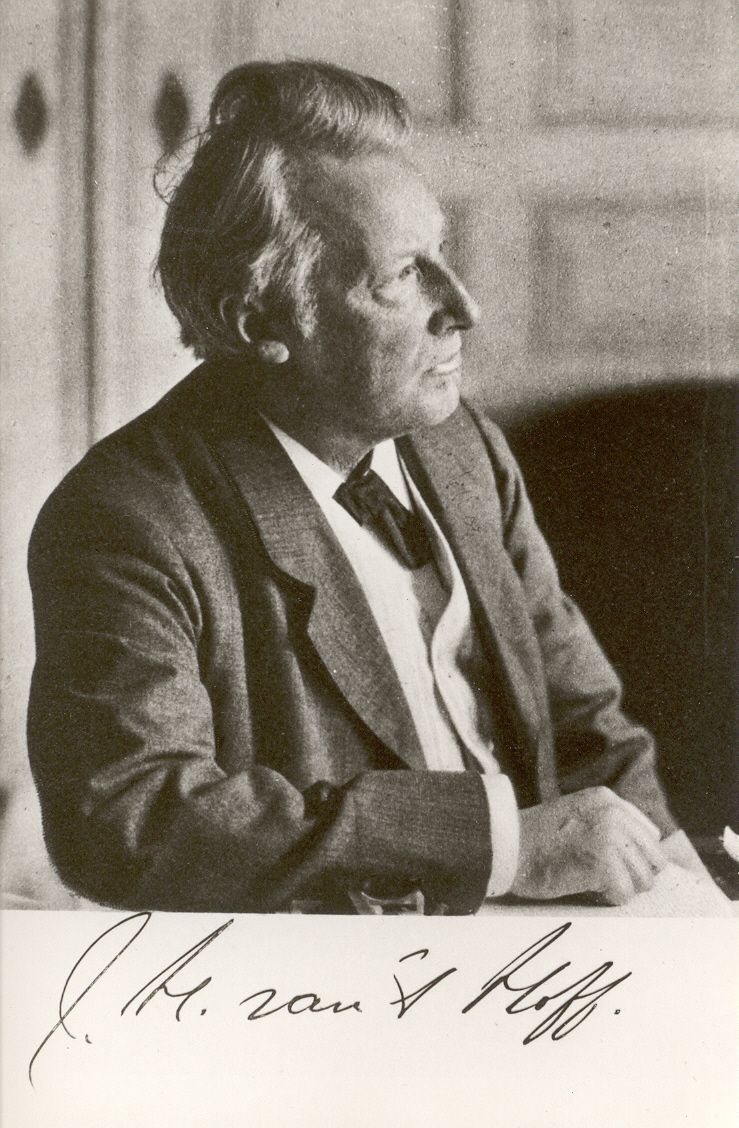
\includegraphics[width=\linewidth]{images/book2/van-t-hoff.jpg}
\end{minipage}\hfill
\begin{minipage}[t]{0.76\linewidth}\vspace{0pt}
Jacobus Henricus van 't Hoff stelde als jonge chemicus voor dat de vier
bindingen van een koolstofatoom naar de hoekpunten van een tetraëder
wijzen. Een koolstofatoom met vier verschillende substituenten bestaat
dan als twee schikkingen die elkaars spiegelbeeld zijn, wat verklaarde
waarom sommige verbindingen in twee vormen voorkomen die alleen
verschillen in de manier waarop ze gepolariseerd licht draaien. Het idee
is het vertrekpunt van elke tekening in dit hoofdstuk.
(Foto gepubliceerd in 1911, publiek domein, Wikimedia Commons.)
\end{minipage}
\end{history}

\section{Conformaties}

\begin{definition}[Torsiehoek en conformaties]\label{def:b1:stereochemistry-in-depth:conformations}
Voor vier atomen A--B--C--D is de \emph{torsiehoek}\index{torsiehoek}
$\theta$ om B--C de hoek tussen de vlakken ABC en BCD, afgelezen op een
\omterm{def:b1:stereochemistry-in-depth:representations}{newmanprojectie} langs B--C. Een \omterm{def:b1:stereochemistry-in-depth:isomers}{conformatie} is een
\emph{eclipsconformatie}\index{eclipsconformatie} wanneer de bindingen
van het voorste en het achterste koolstofatoom in projectie op één lijn
liggen, een \emph{gestaffelde
conformatie}\index{gestaffelde conformatie} wanneer ze afwisselen. In
butaan, bekeken langs C2--C3, is de gestaffelde \omterm{def:b1:stereochemistry-in-depth:isomers}{conformatie} met de twee
methylgroepen op $180^\circ$ de
\emph{anticonformatie}\index{anticonformatie}, die met de methylgroepen
op $\pm 60^\circ$ zijn
\emph{gaucheconformaties}\index{gaucheconformatie}. In cyclohexaan is de
spanningsvrije geplooide ring de \emph{stoel}\index{stoel}; elk
koolstofatoom draagt één \emph{axiale}\index{axiale} binding, evenwijdig
aan de as van de ring, en één
\emph{equatoriale}\index{equatoriale} binding, ruwweg in het gemiddelde
vlak van de ring. De \emph{ringflip}\index{ringflip} zet de ene stoel om
in de andere, waarbij elke axiale binding equatoriaal wordt en omgekeerd.
\end{definition}

\begin{omfigure}
\begin{tikzpicture}
\begin{axis}[
  width=0.82\linewidth, height=5.8cm, xmin=0, xmax=360, ymin=0, ymax=21,
  legend style={font=\scriptsize, draw=none, at={(0.5,0.62)}, anchor=center},
  axis x line=bottom, axis y line=left, xlabel={torsiehoek $\theta$ (graden)},
  ylabel={energie (kJ/mol)}, xtick={0,60,120,180,240,300,360},
  tick label style={font=\small}, label style={font=\small}]
\addplot[omDef, very thick] table[x=theta, y=butane] {figdata/out/bachelor-1-butane-torsion.dat};
\addplot[omProp, thick, dashed] table[x=theta, y=ethane] {figdata/out/bachelor-1-butane-torsion.dat};
\node[font=\scriptsize, anchor=south west] at (axis cs:0,18.4) {syn};
\node[font=\scriptsize, anchor=south] at (axis cs:62,18.4) {gauche};
\node[font=\scriptsize, anchor=south] at (axis cs:120,18.4) {eclips};
\node[font=\scriptsize, anchor=south] at (axis cs:180,18.4) {anti};
\node[font=\scriptsize, anchor=south] at (axis cs:240,18.4) {eclips};
\node[font=\scriptsize, anchor=south] at (axis cs:298,18.4) {gauche};
\node[font=\scriptsize, anchor=south east] at (axis cs:360,18.4) {syn};
\legend{butaan, ethaan}
\end{axis}
\end{tikzpicture}

{\small Torsie-energie van butaan om zijn centrale binding (volle lijn;
$\theta
= 0$ wanneer de methylgroepen elkaar bedekken) en van ethaan (gestreept),
berekend uit experimentele torsiepotentialen. Ethaan: barrière
\qty{12.2}{kJ/mol}. Butaan: anti het stabielst; gauche
\qty{2.8}{kJ/mol} hoger, bij $\theta = 62^\circ$; barrières
\qty{15.2}{kJ/mol} (methyl tegenover waterstof) en \qty{16.5}{kJ/mol}
(methyl tegenover methyl).}
% ledger: rot:ethane-V3, rot:butane-V1, rot:butane-V2, rot:butane-V3, rot:butane-V4, rot:butane-V5, rot:butane-V6 (curves in figdata/bachelor-1/butane-torsion.py)
\end{omfigure}

De barrières zijn klein vergeleken met de thermische energie die bij
botsingen beschikbaar is ($RT = \qty{2.5}{kJ/mol}$ bij kamertemperatuur,
en veel meer in de staart van de verdeling,
\cref{ch:b1:elementary-steps}): de rotatie is snel, en butaan is een
mengsel van anti- en gauchemoleculen dat niet gescheiden kan worden.

\begin{method}[Een stoel tekenen]\label{met:b1:stereochemistry-in-depth:draw-chair}
\begin{enumerate}
  \item Teken twee evenwijdige lijnen die licht naar rechts omlaag
        hellen, ten opzichte van elkaar verschoven; verbind hun uiteinden
        met een V links en een omgekeerde V rechts om de zesring te
        sluiten.
  \item \omterm{def:b1:stereochemistry-in-depth:conformations}{Axiale} bindingen zijn verticaal: omhoog op de koolstofatomen die
        omhoog wijzen, omlaag op die die omlaag wijzen, afwisselend rond
        de ring.
  \item \omterm{def:b1:stereochemistry-in-depth:conformations}{Equatoriale} bindingen zijn evenwijdig aan de ringbindingen die één
        plaats verder liggen, en wijzen naar buiten.
  \item Teken voor een \omterm{def:b1:stereochemistry-in-depth:conformations}{ringflip} de andere \omterm{def:b1:stereochemistry-in-depth:conformations}{stoel}; een substituent die in de
        ene \omterm{def:b1:stereochemistry-in-depth:conformations}{axiaal} staat, staat in de andere \omterm{def:b1:stereochemistry-in-depth:conformations}{equatoriaal}.
\end{enumerate}
\end{method}

\begin{omfigure}
\begin{tikzpicture}[font=\small]
  \pic (a) at (0,0) {omchair};
  \foreach \k in {1,2,3,4,5,6} \draw[omProp, thick] (a-c\k) -- (a-a\k);
  \foreach \k in {1,2,3,4,5,6} \draw[omDef, thick] (a-c\k) -- (a-e\k);
  \node[omProp, anchor=south] at (a-a3) {axiaal};
  \node[omDef, anchor=north] at (a-e5) {equatoriaal};
  \begin{scope}[xshift=4.9cm]
    \pic (b) at (0,0) {omchair};
    \draw[thick] (b-c1) -- (b-e1) node[right] {\ce{CH3}};
    \draw[thick] (b-c1) -- (b-a1) node[above] {H};
    \node at (0,-1.5) {equatoriaal \ce{CH3}};
  \end{scope}
  \draw[<->, thick] (8.1,0) -- (8.8,0) node[midway, above] {flip};
  \begin{scope}[xshift=10.45cm]
    \pic (c) at (0,0) {omchairflip};
    \draw[thick] (c-c4) -- (c-a4) node[below] {\ce{CH3}};
    \draw[thick] (c-c4) -- (c-e4) node[right] {H};
    \node at (0,-1.5) {axiaal \ce{CH3}};
  \end{scope}
\end{tikzpicture}

{\small Links: de \omterm{def:b1:stereochemistry-in-depth:conformations}{stoel} van cyclohexaan met zijn zes \omterm{def:b1:stereochemistry-in-depth:conformations}{axiale} bindingen
(oranje, afwisselend omhoog en omlaag) en zes \omterm{def:b1:stereochemistry-in-depth:conformations}{equatoriale} bindingen
(blauw). Rechts: de twee \omterm{def:b1:stereochemistry-in-depth:conformations}{stoelen} van methylcyclohexaan, die door de
\omterm{def:b1:stereochemistry-in-depth:conformations}{ringflip} in elkaar overgaan; de methylgroep staat in de ene \omterm{def:b1:stereochemistry-in-depth:conformations}{equatoriaal},
in de andere \omterm{def:b1:stereochemistry-in-depth:conformations}{axiaal}.}
\end{omfigure}

\begin{proposition}[Equatoriale substituenten hebben de voorkeur]\label{prop:b1:stereochemistry-in-depth:chair-substituent}
In een monogesubstitueerd cyclohexaan is de \omterm{def:b1:stereochemistry-in-depth:conformations}{stoel} met de substituent
\omterm{def:b1:stereochemistry-in-depth:conformations}{equatoriaal} de stabielste. Voor een methylgroep voegt de axiale positie
twee gauche-interacties met koolstofatomen van de ring toe, elk zo groot
als die in butaan (\qtyrange{2.8}{2.9}{kJ/mol}), samen ongeveer
\qty{5.7}{kJ/mol}: een schatting van het energieverschil.
\end{proposition}

\begin{proof}
Bekeken langs de binding C1--C2 staat een \omterm{def:b1:stereochemistry-in-depth:conformations}{axiale} methylgroep op C1 gauche
ten opzichte van C3 van de ring; bekeken langs C1--C6 gauche ten opzichte
van C5: twee butaanachtige gauche-interacties, die ook gezien worden als
het gedrang van de methylgroep met de \omterm{def:b1:stereochemistry-in-depth:conformations}{axiale} waterstofatomen op C3 en C5
(de 1,3-diaxiale interacties). Een \omterm{def:b1:stereochemistry-in-depth:conformations}{equatoriale} methylgroep staat anti ten
opzichte van C3 en C5. Elke gauche-interactie kost wat ze in butaan kost,
\qty{2.8}{kJ/mol} in de torsiepotentiaal van de figuur.
\end{proof}

Met $\Delta E = \qty{5.7}{kJ/mol}$ is de verhouding van \omterm{def:b1:stereochemistry-in-depth:conformations}{equatoriale} tot
\omterm{def:b1:stereochemistry-in-depth:conformations}{axiale} \omterm{def:b1:stereochemistry-in-depth:conformations}{stoelen} bij \qty{25}{\celsius} gelijk aan $\exp(\Delta E/RT) = 10$:
ongeveer \qty{91}{\percent} \omterm{def:b1:stereochemistry-in-depth:conformations}{equatoriaal}
(\cref{exo:b1:stereochemistry-in-depth:9}). Grote groepen, zoals
tert-butyl, vergrendelen de ring in de \omterm{def:b1:stereochemistry-in-depth:conformations}{stoel} waarin ze \omterm{def:b1:stereochemistry-in-depth:conformations}{equatoriaal} staan.

\section{Optische activiteit}

\begin{definition}[Optische activiteit, specifieke rotatie]\label{def:b1:stereochemistry-in-depth:optical-activity}
Een stof vertoont \emph{optische activiteit}\index{optische activiteit}
als ze het polarisatievlak van lineair gepolariseerd licht dat erdoorheen
gaat, draait. Gezien door een waarnemer die naar het licht kijkt, draait
een \emph{rechtsdraaiende}\index{rechtsdraaiend} stof, geschreven $(+)$,
het met de wijzers van de klok mee, een
\emph{linksdraaiende}\index{linksdraaiend} stof, $(-)$, tegen de wijzers
van de klok in. De \emph{specifieke rotatie}\index{specifieke rotatie}
is $[\alpha] = \alpha/(\ell c)$, waarin $\alpha$ de gemeten
hoek in graden is, $\ell$ de weglengte in decimeter en $c$ de
massaconcentratie in \unit{g/mL}; ze hangt af van de golflengte (meestal
de gele natriumlijn), de temperatuur en het oplosmiddel.
\end{definition}

\begin{omfigure}
\begin{tikzpicture}[font=\small, >={Stealth}]
  \fill[yellow!70!orange] (0,0) circle (0.25);
  \node[below] at (0,-0.45) {lamp};
  \draw[thick] (1.3,-0.7) rectangle (1.45,0.7); \node[below] at (1.37,-0.75) {polarisator};
  \draw[omDef!20, fill=omDef!10] (2.4,-0.45) rectangle (5.6,0.45);
  \node at (4.0,0) {monster, lengte $\ell$};
  \draw[thick] (6.5,-0.7) rectangle (6.65,0.7); \node[below] at (6.57,-0.75) {analysator};
  \draw (7.6,0) circle (0.3); \node[below] at (7.6,-0.45) {oog};
  \draw[->, orange!80!black] (0.3,0) -- (1.25,0);
  \draw[->, orange!80!black] (1.5,0) -- (2.35,0);
  \draw[->, orange!80!black] (5.65,0) -- (6.45,0);
  % polarisation planes
  \draw[thick, omThm] (1.9,-0.35) -- (1.9,0.35);
  \draw[thick, omThm] (6.05,-0.33) -- ++(70:0.0) -- (5.93,0.33);
  \draw[->, omThm] (5.75,0.55) arc[start angle=100, end angle=70, radius=0.6];
  \node[omThm, above] at (6.1,0.75) {$\alpha$};
\end{tikzpicture}

{\small Een polarimeter. De polarisator laat licht door dat in één vlak
trilt; het \omterm{def:b1:stereochemistry-in-depth:stereocentre}{chirale} monster draait dat vlak over $\alpha$; de analysator
wordt gedraaid tot het licht opnieuw uitgedoofd is, wat $\alpha$ meet.}
\end{omfigure}

\begin{proposition}[Wet van Biot]\label{prop:b1:stereochemistry-in-depth:biot}
Voor een verdunde oplossing van meerdere optisch actieve opgeloste stoffen
is de draaiingshoek additief, $\alpha = \ell\sum_i [\alpha]_i c_i$ (de
\emph{wet van Biot}\index{wet van Biot}). Twee \omterm{def:b1:stereochemistry-in-depth:enantiomers}{enantiomeren} hebben
tegengestelde \omterm{def:b1:stereochemistry-in-depth:optical-activity}{specifieke rotaties}; een \omterm{def:b1:stereochemistry-in-depth:enantiomers}{racemisch mengsel} draait het licht
niet.
\end{proposition}

\begin{proof}
In verdunde oplossing draagt elke opgeloste stof onafhankelijk bij,
evenredig met het aantal doorlopen moleculen, dus met $\ell c_i$; dat is
de experimentele inhoud van de wet. Een spiegeling verandert ``met de
klok mee'' in ``tegen de klok in'': het spiegelbeeldmolecuul draait het
vlak over de tegengestelde hoek, en in een \omterm{def:b1:stereochemistry-in-depth:enantiomers}{racemisch mengsel} heffen de
twee bijdragen elkaar op.
\end{proof}

Voor een mengsel van twee \omterm{def:b1:stereochemistry-in-depth:enantiomers}{enantiomeren} met totale concentratie $c$ geeft
de fractie $x$ van de $(-)$-vorm $\alpha = \ell c[\alpha]_{(-)}(x - (1 - x)) =
\ell c[\alpha]_{(-)}(2x - 1)$: $\alpha$ meten geeft de samenstelling. De
optische rotatie hangt op geen eenvoudige manier samen met de
descriptor: een \cip{R}-verbinding kan $(+)$ of $(-)$ zijn; het
\cip{R}-carvon van groene munt is \omterm{def:b1:stereochemistry-in-depth:optical-activity}{linksdraaiend}.

\section{Oefeningen}

\begin{exercise}[$\star$]\label{exo:b1:stereochemistry-in-depth:1}
Deel elk paar in als \omterm{def:b1:stereochemistry-in-depth:isomers}{constitutie-isomeren}, \omterm{def:b1:stereochemistry-in-depth:enantiomers}{enantiomeren}, \omterm{def:b1:stereochemistry-in-depth:enantiomers}{diastereomeren}
of twee \omterm{def:b1:stereochemistry-in-depth:isomers}{conformaties} van één verbinding: butaan-1-ol en butaan-2-ol;
\cip{R}- en \cip{S}-butaan-2-ol; \cip{Z}- en \cip{E}-but-2-een; de
anti- en de \omterm{def:b1:stereochemistry-in-depth:conformations}{gaucheconformatie} van butaan; \cip{R,R}- en
\cip{R,S}-wijnsteenzuur.
\end{exercise}

\begin{exercise}[$\star$]\label{exo:b1:stereochemistry-in-depth:2}
Rangschik met de \omterm{def:b1:stereochemistry-in-depth:cip}{CIP-regels}: \ce{-OH}, \ce{-NH2}, \ce{-CH3}, \ce{-H};
daarna \ce{-CH2OH}, \ce{-CHO}, \ce{-COOH}, \ce{-CH(CH3)2}; daarna
\ce{-Cl}, \ce{-CH2Cl}, \ce{-CCl3}, \ce{-Br}.
\end{exercise}

\begin{exercise}[$\star$]\label{exo:b1:stereochemistry-in-depth:3}
Hoeveel \omterm{def:b1:stereochemistry-in-depth:isomers}{stereo-isomeren} hebben 2,3-dichloorbutaan,
2-broom-3-chloorbutaan en pentaan-2,4-diol? Wijs de mesovormen aan.
\end{exercise}

\begin{exercise}[$\star$]\label{exo:b1:stereochemistry-in-depth:4}
Rangschik de vier substituenten van C5 van carvon met de \omterm{def:b1:stereochemistry-in-depth:cip}{CIP-regels} en
controleer de descriptoren die in de figuur van de twee carvonen
gegeven worden (volle wig: de isopropenylgroep naar de lezer toe, H van
de lezer af).
\end{exercise}

\begin{exercise}[$\star\star$]\label{exo:b1:stereochemistry-in-depth:5}
Teken de \omterm{def:b1:stereochemistry-in-depth:representations}{newmanprojecties} van butaan langs C2--C3 bij $\theta = 0$, 60,
120 en $180^\circ$ en lees hun energieën af op de kromme. Welke fractie
van de moleculen zou gauche zijn als de gauche- en de anti-energie gelijk
waren?
\end{exercise}

\begin{exercise}[$\star\star$]\label{exo:b1:stereochemistry-in-depth:6}
Teken de \omterm{def:b1:stereochemistry-in-depth:representations}{fischerprojectie} van \cip{S}-alanine,
\ce{H2N-CH(CH3)-COOH}, met de zuurgroep bovenaan. Aan welke kant staat de
aminogroep?
\end{exercise}

\begin{exercise}[$\star\star$]\label{exo:b1:stereochemistry-in-depth:7}
Toon aan dat \textit{cis}-1,2-dimethylcyclohexaan in beide \omterm{def:b1:stereochemistry-in-depth:conformations}{stoelen} één
methylgroep \omterm{def:b1:stereochemistry-in-depth:conformations}{axiaal} en één \omterm{def:b1:stereochemistry-in-depth:conformations}{equatoriaal} heeft, terwijl het
\textit{trans}-isomeer een \omterm{def:b1:stereochemistry-in-depth:conformations}{stoel} heeft met beide \omterm{def:b1:stereochemistry-in-depth:conformations}{equatoriaal}. Welk
isomeer is het stabielst? Gebruik de schatting van het hoofdstuk.
\end{exercise}

\begin{exercise}[$\star\star$]\label{exo:b1:stereochemistry-in-depth:8}
Een oplossing van een \omterm{def:b1:stereochemistry-in-depth:stereocentre}{chirale} verbinding van \qty{0.100}{g/mL} in een
buis van \qty{2.00}{dm} draait het licht over $+13.2^\circ$. Bereken
$[\alpha]$. Wat zou een buis van \qty{1.00}{dm} geven? En het \omterm{def:b1:stereochemistry-in-depth:enantiomers}{enantiomeer}
bij dezelfde concentratie?
\end{exercise}

\begin{exercise}[$\star\star$]\label{exo:b1:stereochemistry-in-depth:9}
Bereken met $\Delta E = \qty{5.7}{kJ/mol}$ en de boltzmannverhouding
$\exp(\Delta E/RT)$ de fractie \omterm{def:b1:stereochemistry-in-depth:conformations}{stoelen} van methylcyclohexaan met een
\omterm{def:b1:stereochemistry-in-depth:conformations}{equatoriale} methylgroep bij \qty{25}{\celsius} en bij
\qty{-50}{\celsius}.
\end{exercise}

\begin{exercise}[$\star\star\star$]\label{exo:b1:stereochemistry-in-depth:10}
Leg uit waarom ethaan één soort \omterm{def:b1:stereochemistry-in-depth:conformations}{gestaffelde conformatie} heeft en butaan
er twee (anti en gauche), en waarom gauche minder stabiel is. Schat met
de energieën van de figuur de populatieverhouding anti : gauche van
butaan bij \qty{25}{\celsius} (twee \omterm{def:b1:stereochemistry-in-depth:conformations}{gaucheconformaties}, één anti).
\end{exercise}

\begin{exercise}[$\star\star\star$]\label{exo:b1:stereochemistry-in-depth:11}
Bekijk 2,3,4-trihydroxypentaandizuur,
\ce{HOOC-CH(OH)-CH(OH)-CH(OH)-COOH}. Tel zijn \omterm{def:b1:stereochemistry-in-depth:stereocentre}{stereogene centra}, toon aan
dat het centrale koolstofatoom alleen stereogeen is wanneer de twee
buitenste tegengestelde descriptoren hebben (pseudo-asymmetrisch), en
tel de \omterm{def:b1:stereochemistry-in-depth:isomers}{stereo-isomeren} (meso inbegrepen).
\end{exercise}

\begin{exercise}[$\star\star\star$]\label{exo:b1:stereochemistry-in-depth:12}
Een monster van één \omterm{def:b1:stereochemistry-in-depth:enantiomers}{enantiomeer} van een verbinding ($[\alpha] = +66.0^\circ$
voor de zuivere verbinding onder de gebruikte omstandigheden) is
gedeeltelijk geracemiseerd: bij \qty{0.050}{g/mL} in een buis van
\qty{1.00}{dm} geeft het $+2.31^\circ$. Bereken de fracties van de twee
\omterm{def:b1:stereochemistry-in-depth:enantiomers}{enantiomeren}.
\end{exercise}

\section{Probleem: menthol, het verkoelende molecuul}

\begin{problem}[{Weekendprobleem --- de drie stereocentra van menthol,
zijn acht stereo-isomeren, de stoel met alles equatoriaal, de wet van
Biot, en het percentage (\textminus)-menthol in een gedeeltelijk
geracemiseerd monster}]
\label{pb:b1:stereochemistry-in-depth:1}
Menthol, 2-isopropyl-5-methylcyclohexaan-1-ol, geeft munt zijn
verkoelende gevoel. De natuurlijke verbinding is $(-)$-menthol, met
\omterm{def:b1:stereochemistry-in-depth:isomers}{configuratie} \cip{1R,2S,5R}. Een laboratorium meet met een polarimeter
(natriumlijn, \qty{25}{\celsius}, ethanol, $\ell = \qty{1.00}{dm}$): zijn
referentiemonster van zuiver $(-)$-menthol bij $c = \qty{0.0500}{g/mL}$
geeft $\alpha =
-2.46^\circ$; een te testen monster, bij dezelfde concentratie, geeft
$-1.97^\circ$.

\medskip
\noindent\textbf{Deel I --- Stereocentra.}
\begin{enumerate}
  \item Teken de constitutie van menthol en duid de stereogene
        koolstofatomen aan.
  \item Hoeveel \omterm{def:b1:stereochemistry-in-depth:isomers}{stereo-isomeren} kunnen er zijn? Hoeveel paren
        \omterm{def:b1:stereochemistry-in-depth:enantiomers}{enantiomeren}?
  \item Waarom is er geen mesovorm?
  \item Rangschik de substituenten van C1 met de \omterm{def:b1:stereochemistry-in-depth:cip}{CIP-regels}.
  \item Rangschik de substituenten van C2.
  \item Rangschik de substituenten van C5.
  \item Schrijf de \omterm{def:b1:stereochemistry-in-depth:isomers}{configuratie} van het \omterm{def:b1:stereochemistry-in-depth:enantiomers}{enantiomeer} van $(-)$-menthol op.
\end{enumerate}

\medskip
\noindent\textbf{Deel II --- De \omterm{def:b1:stereochemistry-in-depth:conformations}{stoel}.}
\begin{enumerate}[resume]
  \item Teken een \omterm{def:b1:stereochemistry-in-depth:conformations}{stoel} van cyclohexaan en plaats de drie substituenten
        van $(-)$-menthol allemaal \omterm{def:b1:stereochemistry-in-depth:conformations}{equatoriaal}. Controleer dat dit
        overeenkomt met de relatieve schikking (1,2-\textit{trans} en
        1,5-\textit{cis}) van menthol.
  \item Wat gebeurt er met de drie substituenten in de omgeklapte \omterm{def:b1:stereochemistry-in-depth:conformations}{stoel}?
  \item Leg met de schatting van het hoofdstuk voor één \omterm{def:b1:stereochemistry-in-depth:conformations}{axiale}
        methylgroep uit waarom menthol bijna volledig in één \omterm{def:b1:stereochemistry-in-depth:conformations}{stoel}
        voorkomt.
  \item Neomenthol verschilt alleen bij C1 van menthol. Is het een
        \omterm{def:b1:stereochemistry-in-depth:enantiomers}{enantiomeer} of een \omterm{def:b1:stereochemistry-in-depth:enantiomers}{diastereomeer} van menthol?
  \item Welke groep staat \omterm{def:b1:stereochemistry-in-depth:conformations}{axiaal} in de beste \omterm{def:b1:stereochemistry-in-depth:conformations}{stoel} van neomenthol?
  \item Waarom hebben menthol en neomenthol verschillende kookpunten, en
        de twee \omterm{def:b1:stereochemistry-in-depth:enantiomers}{enantiomeren} van menthol niet?
\end{enumerate}

\medskip
\noindent\textbf{Deel III --- Optische rotatie.}
\begin{enumerate}[resume]
  \item Bereken $[\alpha]$ van het referentiemonster. Vergelijk met het
        bereik van $-45^\circ$ tot $-51^\circ$ dat een handboek voor
        $(-)$-menthol geeft.
  \item Wat zou $[\alpha]$ van $(+)$-menthol zijn? En van racemisch
        menthol?
  \item Bereken $[\alpha]$ van het geteste monster.
  \item Schrijf de \omterm{prop:b1:stereochemistry-in-depth:biot}{wet van Biot} op voor een mengsel van de twee
        \omterm{def:b1:stereochemistry-in-depth:enantiomers}{enantiomeren}, met $x$ de fractie $(-)$-menthol.
  \item Druk $x$ uit als functie van de gemeten rotatie en de
        referentierotatie.
  \item Kan een \omterm{def:b1:stereochemistry-in-depth:stereocentre}{chirale} verontreiniging van een andere verbinding de
        meting vertekenen? Geef een controle.
\end{enumerate}

\medskip
\noindent\textbf{Deel IV --- De samenstelling.}
\begin{enumerate}[resume]
  \item Bereken de fractie $(-)$-menthol in het geteste monster.
  \item Het monster van een tweede leverancier geeft onder dezelfde
        omstandigheden $-2.40^\circ$. Bereken de samenstelling ervan.
  \item Welk monster ligt het dichtst bij natuurlijk menthol?
  \item Welke hoek zou het geteste monster geven met een buis van
        \qty{2.00}{dm}, en waarom is een langere buis beter?
  \item Geef het percentage $(-)$-menthol in het geteste monster, op drie
        beduidende cijfers.
\end{enumerate}
\end{problem}
